% ============================================================
%  第五卷 第一章 统计物理学的基本原理（§1–§8）
%  底本：高教社中文版第5版（束仁贵/束莼 译，郑伟谋 校）
%  本章插图 1 幅（图1，§8）；无习题（与原书一致）；
%  正文圈码 19 处已全部还原为 \footnote（脚注代理转录，页码 p3–p27，含
%  \mathfrak{O}→①的 δ 函数脚注；p14 ①与 p17 ①脚注内含 equation* 展式，
%  其中 (5.10a) 为脚注内带 \tag 的编号式，与原书一致）。
%  已修正的 OCR/原书错误（均对照 原书转换/pages/p-017…p-042.png 核实）：
%   1. 大写 Γ 被 OCR 误作 T：dΓ、ΔΓ、Γ(E) 及 (6.5)(7.1)(7.3)(7.4)(7.6)
%      (7.7)(7.8)(7.13)(7.15) 诸式中的统计权重/态数一律还原为 Γ。
%   2. 微正则分布的常数因子 OCR 乱码（\stackrel{\varkappa}{\eta}^*3…、
%      \frac{2\pi}{13}\frac{3\pi}{3}\alpha、\breve{H}_3^*H\times、
%      \mathbf{\Pi}_H^{at}\frac{*w}{\hbar}\mathcal{K}\hat{B} 等）按原书
%      p-025/p-026/p-034/p-038/p-039 恢复为"常数·"：(4.4)(4.6)(6.6)及
%      (7.15)前的重复式、(7.16)(7.17)。
%   3. 平均值记号：OCR 把 \bar f 误作 \hat f（§2 相对涨落分母两处、
%      §5 (5.5) 前一处），按原书改为 \bar f；§2 的 ⟨(Δf)²⟩ 尖括号为原书
%      记号（原书 p-019 脚注①声明横线与尖括号两种平均值写法并用），照排。
%   4. (1.1) 分子 Δι→Δt；时间平均公式 lim 中 τ→∞ 按原书统一为 T。
%   5. (1.2) 的 dq_ℓ、§5 的 dq_2（间隔 dq=dq₁dq₂…）下标按原书为 s；
%      (2.3) OCR 掉了尖括号，按原书补为 ⟨(Δf)²⟩=\overline{f^2}-(\bar f)²；
%      (7.9) 前"平均值 ln w(E_n)"按原书补尖括号； (7.12) 首项按原书补
%      ⟨⟩（p-038：S=-⟨ln[(2πħ)^s ρ]⟩=-∫…）。
%   6. (3.2) 求和上限 ^ν→s；§3 各式 v_i=ẋ_i 及 q,p 之粗体系 OCR 噪声，
%      按原书改斜体；(6.1)前后两处 (E_n-E_n)→(E_n-E_m)（原书 p-032/33）。
%   7. (4.4) 前 OCR 乱序"任何函数ρ……ρ并且满足"按原书语序复原；
%      "δ函数\mathfrak{O}的出现"之 \mathfrak{O} 系圈码①误读，还原为①。
%   8. (7.6)(7.8) 的 (2πħ)′、[(erg·s)^*]、(7.8)下文 a′ΔpΔq 的指数一律
%      为 s（p-035/p-037）；(7.16)(7.17) 及 §7/§8 正文的 e^s→e^S。
%   9. 词语修正：引人→引入（两处，原书 p-041 实为"引入"）、
%      扩涨→扩张（原书 p-040 实为"宇宙学扩张"）、"都∴须"→"都必须"。
%  10. 行410/442/466/472/632/650/676/696/1068/1088 等段末句号 OCR 脱落，
%      按原书补齐；§3 末"分布函数保持恒定这就是刘维尔定理"原书脱标点，
%      按文意补逗号（p-024）；OCR 伪段落裂（"给出Γ利用…来/进行计算"、
%      "任意选/定"、"十分微/小"、"完全/无关紧要"）按原书合并。
%  遗留问题：
%   - §8 "玻尔兹曼（L.Boltzmann，1870's）"之"1870's"原书如此（p-040），照排。
%   - 行632"任何物理量的平均值"后原书有句号（已补）；行974"可加常数"原书
%     如此（非"可加性常数"），照排。
%   - 行1030"某个假想中极为巨大的系统"语义存疑但原书 p-038 如此，照排。
% ============================================================
\chapter{统计物理学的基本原理}

\section{统计分布}

统计物理学（或简称统计学）的目的是研究宏观物体的行为和性质所遵循的特殊一类规律性，所谓宏观物体是指由大量的单个粒子（原子、分子）构成的物体.这些规律性的共同特点，在很大程度上与物体中各个粒子的运动用什么力学——经典力学还是量子力学——来描述是无关的；然而，在这两种情形下，这些规律性的论证所要求的方式不同.为叙述方便起见，我们首先在经典力学适用的假设下进行所有的讨论.

写出力学系统的运动方程（其数目等于该系统的自由度的数目），并将其积分，在原则上我们能够得到关于该系统运动的详尽无遗的知识.但是，如果我们必须处理这样的系统——虽然它遵循经典力学的规律，但其自由度的数目却非常巨大，那么在实际应用力学的方法时，我们就必然要写出并求解同样多的微分方程式，以至于实际上是实现不了的.应该着重指出：即使能够把这些微分方程以普遍的形式积分出来，想把所有粒子的速度和坐标的初始条件代入通解中去也是根本不可能的.

乍一看来可以由此得出结论：随着粒子数目的增加，力学系统的性质必定会变得难以想像的复杂和紊乱，以至在宏观物体的行为中我们将不可能找到任何规范性的迹象.然而，情况并非如此，以后我们会看到：在粒子数目相当大的情形下，出现一些新的独特规律性.

这些规律性——所谓的统计规律性——正是以存在大量的构成物体的粒子为其先决条件，决不可能把它们归结为纯粹的力学规律性.这些规律的特点表现在：当它们应用到自由度数目不大的力学系统时，它们便失去任何意义.因此，具有巨大自由度数目的系统的运动虽然与粒子数不多的系统的运动遵循同样的力学规律，但是自由度数目的巨大却导致性质上全新的规律性.

统计物理学在理论物理学诸多分支中的重要价值就在于：在自然界中我们经常遇到的总是宏观物体，它们的行为根据上述的原因不可能用纯粹力学的方法作详尽的描述，它们服从的是统计的规律性.

为表述经典统计学的基本问题，我们首先要引入“相空间”的概念，这是以后经常用到的概念.

设我们所考虑的宏观力学系统有 $s$ 个自由度.换而言之，这个系统的各点在空间的位置由 $s$ 个坐标来表征，我们用字母 $q_i$ 表示这些坐标，角标 $i$ 取 $1,2,\cdots,s$ 诸值.那么在给定时刻系统的状态将取决于该时刻的 $s$ 个坐标 $q_i$ 以及 $s$ 个与之相应的速度 $\dot{q}_i$ 的值.在统计学中通常用系统的坐标 $q_i$ 与动量 $p_i$（而不用速度）来表征系统的状态，因为这样做有很大的优越性.系统的不同状态在数学上可以用相空间（当然这纯粹是数学上的概念）中不同的点来表示；在这个空间的坐标轴上标出的是该系统的坐标值与动量值.因此，每个系统有自己独特的相空间，该相空间的维数等于系统自由度数的两倍.相空间的每一点，对应于系统一组确定坐标值 $q_i$ 与动量值 $p_i$，因而代表这个系统的一个确定的状态.系统的状态随着时间而变化，相应地，表示系统相空间中状态的点（以后我们把它简称为“系统的相点”）将在相空间中描画出一条曲线，称为相轨道.

现在我们来考虑任意的宏观物体或物体系统.假设系统是闭合的，即该系统与任何其它物体都不产生相互作用.设想从这个系统中划分出某一部分，它与整个系统相比非常小，然而它又是宏观的；显然，当整个系统中的粒子数足够大时，在它的一小部分中的粒子数仍然可以很大.这种相对很小却又是宏观的部分称为子系统.子系统仍然是力学系统，但绝不是闭合的，相反，它经受到来自系统其余各部分所有可能的作用.由于这些其余部分的自由度数量巨大，这种相互作用具有十分复杂而又紊乱的特征.因而子系统的状态随着时间以非常复杂而紊乱的方式变化.

要精确求解关于子系统的行为问题，只有通过求解整个闭合系统的力学问题的办法，即通过写出并在给定初始条件下求解全部微分运动方程组的办法；正如已经指出的，这是一个无法实现的问题.幸而，正是由于子系统状态的这种极其复杂变化过程使力学的方法不再适用，但却给出了从另一方面求解问题的可能性.

这一见解的根据在于：由于被我们划分出来的子系统与系统的其余各部分间的相互作用极其复杂而紊乱，在足够长的时间间隔内子系统在自身所有可能的状态中经历足够多的次数.

更精确地讲，这个情况应当表述如下.我们用 $\Delta p\,\Delta q$ 表示子系统的相空间中某个小区域的“体积”，对应于子系统的坐标 $q_i$ 和动量 $p_i$ 的值位于小间隔 $\Delta q_i$ 与 $\Delta p_i$ 内.可以确信，在足够长的时间 $T$ 内，子系统的十分紊乱的相轨道会多次穿过相空间中每一个这样的区域.设在总时间 $T$ 内，子系统“处于”相空间中给定区域 $\Delta p\,\Delta q$ 内\footnote{为简短起见，通常我们按照习惯说成：系统“处于相空间的区域 $\Delta p\,\Delta q$ 中”，这时所指的是：系统处于用在这一区域的相点所表示的状态中.}那一段时间为 $\Delta t$.当总时间 $T$ 无限增大时，比值 $\Delta t/T$ 将趋于某个极限值
\begin{equation}
  \omega=\lim_{T\to\infty}\frac{\Delta t}{T}.
\end{equation}
显然，可以把这个数值看成是当我们在某个任意时刻观测子系统时发现它处于相空间中给定区域 $\Delta p\,\Delta q$ 内的概率.

当相空间中的体积元\footnote{以后我们总是约定用 $\mathrm{d}p$ 和 $\mathrm{d}q$ 分别表示系统的全部动量微分的乘积和全部坐标微分的乘积.}变为无限小时，
\begin{equation}
  \mathrm{d}q\,\mathrm{d}p=\mathrm{d}q_1\mathrm{d}q_2\cdots\mathrm{d}q_s\,\mathrm{d}p_1\mathrm{d}p_2\cdots\mathrm{d}p_s,
\end{equation}
我们可以引入 $\mathrm{d}\omega$ 来表示由这个体积元中的相点所代表的状态的概率，即坐标 $q_i$ 与动量 $p_i$ 的值位于给定的 $q_i,p_i$ 与 $q_i+\mathrm{d}q_i,\ p_i+\mathrm{d}p_i$ 之间的无限小的间隔内的概率，这个概率 $\mathrm{d}\omega$ 可以写成
\begin{equation}
  \mathrm{d}\omega=\rho(p_1,\cdots,p_s,q_1,\cdots,q_s)\,\mathrm{d}p\,\mathrm{d}q,
\end{equation}
式中 $\rho(p_1,\cdots,p_s,q_1,\cdots,q_s)$ 是全部坐标与全部动量的函数（通常将其简记为 $\rho(p,q)$，甚至简写为 $\rho$).函数 $\rho$ 起着相空间中概率分布“密度”的作用，称为该物体的统计分布函数（或简称分布函数).显然，分布函数应该满足“归一化条件”
\begin{equation}
  \int\rho\,\mathrm{d}p\,\mathrm{d}q=1,
\end{equation}
积分遍及整个相空间.它表明了这样一个简单事实：所有可能的状态的概率之和应当为1.

对统计学而言，最重要的是：某个子系统的统计分布与同一系统的其它任意小部分的初始状态无关，因为这种初始状态的影响在足够长的时间内被系统中其余的更为广大的部分的影响所完全消除.这种被我们划分出来的子系统的统计分布也与它自身的初始状态无关，因为子系统将逐渐经历所有可能的状态，因而其中的每一个状态都可以取作初始状态.因此不必考虑到用初始条件来解决系统的力学问题的办法，就可以求出系统中各个小部的统计分布.

求出任意子系统的统计分布是统计学的基本课题.当我们说闭合系统的各个“小部分”时，应当注意到：我们所需要考虑的宏观物体通常就已经是一个更大的闭合系统的这样的“小部分”，这个更大的闭合系统就是由这些宏观物体同它们周围的外部介质一起构成的.

如果上述问题已经解决，因而该子系统的统计分布已经知道，那么我们就可以把任何依赖于子系统状态的（即依赖于子系统坐标 $q$ 和动量 $p$ 之值的）物理量取不同值的概率计算出来.我们也可以计算出任何这种物理量 $f(p,q)$ 的平均值，只要把它的所有可能值乘以相应的概率，并遍及所有的状态进行积分，就可以得到.我们用在字母上加一横线的办法来表示平均值，于是就可以写出公式
\begin{equation}
  \bar{f}=\int f(p,q)\rho(p,q)\,\mathrm{d}p\,\mathrm{d}q,
\end{equation}
按照这一公式就可以用统计分布函数来计算各种物理量的平均值.\footnote{本书中，我们将用字母加上横线 $\bar{f}$ 或尖括号 $\langle f\rangle$ 表示平均值，这仅仅是为了书写公式方便；为了书写繁冗表达式的平均值，最好采用第二种写法.}

用分布函数来求平均（或者说，统计平均）使我们不必为了确定物理量 $f(p,q)$ 的平均值而去追踪它随时间的真实变化.同时也很明显，正是由于概率概念的定义，按照公式 (1.1)，统计平均完全等价于按时间来求平均.对时间求平均的意思是：如果我们追踪物理量随时间的变化，那么一定能建立起一个函数 $f=f(t)$，然后把所要求的平均值定义为
\begin{equation*}
  \bar{f}=\lim_{T\to\infty}\frac{1}{T}\int_0^{T}f(t)\,\mathrm{d}t.
\end{equation*}

从上面的叙述可知：统计学所能作出的关于宏观物体行为的结论和预言具有概率的特征.这就是统计学不同于（经典）力学之处，后者的结论是具有完全确定的特征的.但是必须着重指出，经典统计学的结论的概率特征绝非它所研究的客体本身所固有，而只是由于得到这些结论所依据的条件远比完整的力学描述所需要的少得多（不需要知道全部坐标和动量的初始值）的缘故.

但是在实际上，在把统计学应用于宏观物体时，它的概率特征通常完全表现不出来.这是因为：如果在足够长的时间间隔内观测任何一个宏观物体（处于稳定的，即与时间无关的外界条件下）就会发现：所有表征这个物体的物理量实际上都是常量（等于它们的平均值），而很少显示出任何明显的偏离.这里所说的“宏观物理量”所表征的是整个物体或者它的各个宏观部分，而不是单个粒子\footnote{我们举一个例子直观地说明这一规则精确到什么程度.若在某种气体中划分出一部分，比如说只有 $1/100$ 摩尔分子，则会发现这部分物质的能量对其平均值的平均偏差是 $\sim10^{-11}$.如果我们想要在一次观测中，发现数量级为 $10^{-6}$ 的相对偏差，那么就会发现这种偏差的概率小得出奇，约为 $10^{-3\times10^{15}}$.}.统计学的这个基本情况是从（将在下一节中阐明的）非常普遍的考虑得出来的，而且所考虑的物体愈复杂、愈庞大，结果就愈正确.用统计分布的术语可以说：如果用函数 $\rho(p,q)$ 来构成一个表示物理量 $f(p,q)$ 取不同值的概率的分布函数，那么这个函数将在 $f=\bar{f}$ 处具有非常陡的极大值，即在最靠近极大值的范围内这个函数才明显地不等于零.

由此可见，由于统计学给出了计算表征宏观物体的物理量平均值的可能性，任意时间间隔只要长到足以消除物体初始状态的影响，那么在这个时间间隔的绝大部分时间内，统计学所作出的预言都是高度正确的.在这个意义下，统计学的预言实际上是确定的，而非概率的.（由于这一点，今后在表示宏观物理量时，几乎总是不在字母上加横线了.）

如果闭合宏观系统在其所处的状态下，其任何宏观子系统的宏观物理量都充分精确地等于相应量的平均值，那么就说系统处于统计平衡状态（也称为热力学平衡或热平衡状态).由上面可以看出：如果在足够长的时间间隔内观测闭合的宏观系统，那么在这个间隔的绝大部分时间内它都是处于统计平衡状态的.不论在任何初始时刻，假如闭合的宏观系统不处在统计平衡状态（例如，人为地对系统施加外作用，使它离开统计平衡状态，然后再把它孤立起来，使它重新成为闭合系统），那么以后一定会过渡到平衡状态.过渡到统计平衡状态所需要的时间称为弛豫时间.我们在上面所说的“足够长”的时间间隔，实质上就是指比弛豫时间长得多的时间间隔.

与过渡到平衡状态有关的过程理论，称为动理学，它本来就不是统计学的研究对象，统计学所研究的是处于统计平衡状态的系统.

\section{统计独立}

在§1中所讲到的子系统本身并不是闭合的.相反，它们受到来自系统中其它部分的连续不断的作用.虽然这些部分比起整个大系统来要小得多，但是它们本身仍然是宏观物体.正因为如此，我们总可以认为在不太长的时间间隔内，它们的行为近似于闭合系统.实际上，子系统中与周围部分发生相互作用的主要是那些在子系统表面附近的粒子.这些粒子的数目与子系统中粒子总数之比随着子系统尺度的增加而迅速下降，因而当子系统足够大时，它与周围部分相互作用的能量比子系统的内能要小得多.因此可以说，子系统是“准闭合”的.但是必须再次强调指出：子系统的准闭合性只在不太长的时间间隔内才能成立.而在足够长的时间间隔内，子系统之间的相互作用不管多么微弱，总会表现出来.不仅如此，统计平衡之得以建立，归根到底就是全靠这些比较微弱的相互作用.

可以认为各个不同的子系统是彼此微弱地相互作用着，这一事实也就相当于：可以把它们认为在统计意义上是独立的.统计独立性意味着：一个子系统所处的状态绝不影响其它子系统处于不同状态的概率.

考虑任意两个子系统，并设 $\mathrm{d}p^{(1)}\mathrm{d}q^{(1)}$ 和 $\mathrm{d}p^{(2)}\mathrm{d}q^{(2)}$ 表示它们的相空间体积元.如果把两个子系统的集合看成一个组合的子系统，那么从数学的观点来看，子系统的统计独立性就意味着：组合子系统处于它的相体积元 $\mathrm{d}p^{(12)}\mathrm{d}q^{(12)}=\mathrm{d}p^{(1)}\mathrm{d}q^{(1)}\cdot\mathrm{d}p^{(2)}\mathrm{d}q^{(2)}$ 中的概率，可以分解为每个子系统分别处于 $\mathrm{d}p^{(1)}\mathrm{d}q^{(1)}$ 和 $\mathrm{d}p^{(2)}\mathrm{d}q^{(2)}$ 中的概率的乘积，并且每个概率仅与该子系统的坐标和动量有关.因此可以写出
\begin{equation*}
  \rho_{12}\mathrm{d}p^{(12)}\mathrm{d}q^{(12)}
  =\rho_1\mathrm{d}p^{(1)}\mathrm{d}q^{(1)}\cdot\rho_2\mathrm{d}p^{(2)}\mathrm{d}q^{(2)},
\end{equation*}
或
\begin{equation}
  \rho_{12}=\rho_1\rho_2,
\end{equation}
其中 $\rho_{12}$ 是组合子系统的统计分布函数，而 $\rho_1$ 和 $\rho_2$ 是单个子系统的统计分布函数；对于几个子系统的集合也可以写出类似的关系式\footnote{当然是在这样的条件下：这些子系统的集合仍然是整个闭合系统的一个小部分.}.

显然它的逆定理也成立：如果某个复合系统的概率分布也可以分解为几个因子的乘积，而每个因子又只与表征复合系统的一部分物理量有关，那么这就表示这些部分是统计独立的，并且每个因子正比于相应部分的状态概率.

如果 $f_1$ 和 $f_2$ 是两个属于不同子系统的物理量，那么从 (2.1) 以及平均值的定义 (1.5) 直接得到：乘积 $f_1f_2$ 的平均值就等于物理量 $f_1$ 和 $f_2$ 的各自平均值的乘积：
\begin{equation}
  \overline{f_1f_2}=\bar{f}_1\cdot\bar{f}_2.
\end{equation}

我们来考察属于某个宏观物体或它的某一部分的任意一个物理量 $f$.该物理量随时间变化，在其平均值附近摆动.现在我们引进一个量，用它来量度这种变化的平均幅度.差值 $\Delta f=f-\bar{f}$ 的平均值不适于这个目的，因为物理量 $f$ 对其平均值的偏差是双向的，差值 $f-\bar{f}$ 时正时负，平均值总是等于零，而不论 $f$ 是如何频繁地显著偏离其平均值.作为偏差程度的量度，最合适的是取这个差值的平方的平均值.因为 $(\Delta f)^2$ 总是正的，因此它的平均值只有当它本身趋于零时才趋于零；换句话说，只有当 $f$ 对 $\bar{f}$ 的明显偏差具有非常小的概率时，$(\Delta f)^2$ 的平均值才会很小.$\sqrt{\left\langle(\Delta f)^2\right\rangle}$ 称为物理量 $f$ 的均方根涨落.把平方值 $(f-\bar{f})^2$ 展开，我们得出
\begin{equation}
  \left\langle(\Delta f)^2\right\rangle=\overline{f^2}-(\bar{f})^2,
\end{equation}
即一个物理量的均方根涨落取决于它的平方的平均值与它的平均值的平方之差.

比值
\begin{equation*}
  \frac{\sqrt{\left\langle(\Delta f)^2\right\rangle}}{\bar{f}}
\end{equation*}
称为 $f$ 这个量的相对涨落.$f$ 这个量对它的平均值的偏差在某种状态中可能达到与平均值本身可以相比的程度，相对涨落愈小，则物体处于这种状态的时间就愈微不足道.

现在我们来证明：物理量的相对涨落随着它们所从属的物体尺度（粒子数）的增加而迅速减小.为了证明这一点，应当预先指出：大多数有物理意义的量都是可加量；这种情况是物体中各个部分的准封闭性的结果，它的意思也就是说：整个物体的这种物理量的值等于它的各个（宏观）部分的该物理量的值之和.例如，物体中各部分的内能（根据上述理由）比它们的相互作用能量大得多，所以整个物体的能量可以足够精确地认为等于它的各部分的能量之和.

设 $f$ 为这种可加的物理量.设想把所考虑的物体分成数目很大的 $N$ 个大致相同的小部分.那么，
\begin{equation*}
  \bar{f}=\sum_{i=1}^{N}\bar{f}_i,
\end{equation*}
其中 $f_i$ 是属于物体各个部分的物理量.

显然，随着物体尺度的增加，$\bar{f}$ 大致与 $N$ 成正比地增长.其次，我们来确定物理量 $f$ 的均方涨落.我们有
\begin{equation*}
  \left\langle(\Delta f)^2\right\rangle
  =\left\langle\Bigl(\sum_{i=1}^{N}\Delta f_i\Bigr)^2\right\rangle.
\end{equation*}
但是，由于物体各部分的统计独立性，乘积的平均值
\begin{equation*}
  \overline{\Delta f_i\cdot\Delta f_k}
  =\overline{\Delta f_i}\cdot\overline{\Delta f_k}=0
  \qquad(i\neq k)
\end{equation*}
（因为每个 $\overline{\Delta f_i}=0$).因此，
\begin{equation}
  \left\langle(\Delta f)^2\right\rangle
  =\sum_{i=1}^{N}\left\langle(\Delta f_i)^2\right\rangle.
\end{equation}
由此得出：当 $N$ 增加时，均方涨落 $\left\langle(\Delta f)^2\right\rangle$ 也将与 $N$ 成正比地增长.而相对涨落与 $\sqrt{N}$ 成反比，即
\begin{equation}
  \frac{\sqrt{\left\langle(\Delta f)^2\right\rangle}}{\bar{f}}
  \propto\frac{1}{\sqrt{N}}.
\end{equation}

从另一方面来看，如果我们约定把均匀物体分成大小一定的许多小块，则显然，这些小块的数目将与物体中的粒子（分子）总数成正比.因此所得的结果也可以如下表述：任何可加量 $f$ 的相对涨落与宏观物体的粒子数的平方根成反比，所以当粒子数足够大时，实际上可以认为 $f$ 这个量本身就是不随时间变化的常量，并且就等于它的平均值.这个结论已经在上一节中用过.

\section{刘维尔定理}

我们现在进一步研究统计分布函数的性质.

假定在一段很长的时间内观测某个子系统.把这段时间划分为大量的（在极限情况下无穷大）同样大小的时间间隔，这些时间间隔的分界点在 $t_1,t_2,\cdots$ 这些时刻.在每一个这样的时刻，所研究的子系统在相空间中由一点来代表（我们把这些点称为 $A_1,A_2,A_3,\cdots$).这样得到的点集合以一定密度分布在相空间中，在极限情形下，相空间每一处的密度都与分布函数 $\rho(p,q)$ 的值成正比，这是因为分布函数本来的意义就是子系统处于各个不同状态的概率.

我们可以不去考察表示单个子系统在不同时刻 $t_1,t_2,\cdots$ 所处状态的相点，而纯粹形式地同时考察大量的（在极限情形是无穷大）、完全等同的子系统\footnote{这种假想的全同系统的集合通常称为统计系综.}，它们在同一时刻（譬如说 $t=0$)分别处于相点 $A_1,A_2,\cdots$ 所代表的状态.

现在我们来追踪代表这些子系统状态的相点以后的运动，但是所考虑的时间间隔不能太长，以使准闭合的子系统可以足够精确地看成是闭合系统.于是相点的运动服从运动方程，这些方程只涉及子系统的粒子坐标和动量.

显然，根据在 $t=0$ 时的同样理由，在任何时刻 $t$，所有这些相点将按照同一个分布函数 $\rho(p,q)$ 分布在相空间中.换句话说，虽然相点随着时间而运动，但是它们在各处的分布密度仍然保持不变，而且与相应的 $\rho$ 值成正比.

可以把相点的这种运动纯粹形式地看成在 $2s$ 维相空间中稳定的“气”流，因而可以对它应用表示气体“粒子”（现在的情形是相点）总数不变的熟悉的连续性方程.通常的连续性方程具有形式
\begin{equation*}
  \frac{\partial\rho}{\partial t}+\nabla\cdot(\rho\boldsymbol{v})=0
\end{equation*}
（$\rho$ 是密度，$\boldsymbol{v}$ 是气体的速度)，而对于稳定的流动有：
\begin{equation*}
  \nabla\cdot(\rho\boldsymbol{v})=0.
\end{equation*}
把上式推广到 $2s$ 维空间情形为
\begin{equation*}
  \sum_{i=1}^{2s}\frac{\partial}{\partial x_i}(\rho v_i)=0.
\end{equation*}
在现在的情形下，“坐标” $x_i$ 是坐标 $q$ 与动量 $p$，而“速度” $v_i=\dot{x}_i$ 是它们对时间的导数 $\dot{q}$ 和 $\dot{p}$，由力学方程所决定.因此，有
\begin{equation*}
  \sum_{i=1}^{s}\left[\frac{\partial}{\partial q_i}(\rho\dot{q}_i)
  +\frac{\partial}{\partial p_i}(\rho\dot{p}_i)\right]=0.
\end{equation*}
把上式导数展开，可以写成
\begin{equation}
  \sum_{i=1}^{s}\left[\dot{q}_i\frac{\partial\rho}{\partial q_i}
  +\dot{p}_i\frac{\partial\rho}{\partial p_i}\right]
  +\rho\sum_{i=1}^{s}\left[\frac{\partial\dot{q}_i}{\partial q_i}
  +\frac{\partial\dot{p}_i}{\partial p_i}\right]=0.
\end{equation}
把力学方程写成哈密顿形式
\begin{equation*}
  \dot{q}_i=\frac{\partial H}{\partial p_i},\qquad
  \dot{p}_i=-\frac{\partial H}{\partial q_i},
\end{equation*}
其中 $H=H(p,q)$ 是所考察的子系统的哈密顿函数，我们看出
\begin{equation*}
  \frac{\partial\dot{q}_i}{\partial q_i}
  =\frac{\partial^2 H}{\partial q_i\partial p_i}
  =-\frac{\partial\dot{p}_i}{\partial p_i}.
\end{equation*}
因此 (3.1) 式中的第二项恒等于零，而第一项不是别的，正是分布函数对时间的全导数，因而我们有
\begin{equation}
  \frac{\mathrm{d}\rho}{\mathrm{d}t}
  =\sum_{i=1}^{s}\left(\frac{\partial\rho}{\partial q_i}\dot{q}_i
  +\frac{\partial\rho}{\partial p_i}\dot{p}_i\right)=0.
\end{equation}
因此，我们得到一个重要的结论：沿着子系统的相轨道，分布函数保持恒定，这就是刘维尔定理.应当注意的是，由于我们所讨论的是准闭合的系统，只有当时间间隔不太长，因而子系统行为可以足够精确地看作是闭合系统时，上面所得到的结果才成立.

\section{能量的作用}

从刘维尔定理可以直接得出结论：分布函数只能表示为变量 $p$，$q$ 的这样一些组合，它们在子系统作为闭合系统而运动时保持不变.这就是所谓的力学不变量或运动积分，众所周知，它们是运动方程式的第一积分.因此可以说，由于分布函数是力学不变量的函数，它本身也是运动积分.

其次，分布函数所可能依赖的运动积分的数目也可以大大减少.为此应当考虑到，两个子系统的集合的分布函数 $\rho_{12}$ 等于这两个子系统各自的分布函数 $\rho_1$ 和 $\rho_2$ 的乘积：$\rho_{12}=\rho_1\rho_2$.因此
\begin{equation}
  \ln\rho_{12}=\ln\rho_1+\ln\rho_2,
\end{equation}
即分布函数的对数是可加性的量.因而我们得出结论：分布函数的对数不仅应该是运动积分，而且应该是可加性的运动积分.

从力学中大家知道，总共存在着七个独立的可加性的运动积分：能量、动量矢量的三个分量和角动量矢量的三个分量.我们分别用 $E_a(p,q),\boldsymbol{P}_a(p,q),\boldsymbol{M}_a(p,q)$ 来表示第 $a$ 个子系统的能量、动量和角动量作为子系统中粒子的坐标和动量的函数.这些量的唯一的可加性组合是以下形式的线性组合：
\begin{equation}
  \ln\rho_a=\alpha_a+\beta E_a(p,q)
  +\boldsymbol{\gamma}\cdot\boldsymbol{P}_a(p,q)
  +\boldsymbol{\delta}\cdot\boldsymbol{M}_a(p,q),
\end{equation}
式中 $\alpha_a,\beta,\boldsymbol{\gamma},\boldsymbol{\delta}$ 是常系数，并且对于给定闭合系统的所有子系统的 $\beta,\boldsymbol{\gamma},\boldsymbol{\delta}$ 应该是相同的.

我们将在以后（第三章）对分布函数 (4.2) 作详细研究.这里对我们重要的只是下面的事实.系数 $\alpha_a$ 就是归一化常数，由条件 $\int\rho_a\,\mathrm{d}p^{(a)}\mathrm{d}q^{(a)}=1$ 来确定.常数 $\beta,\boldsymbol{\gamma},\boldsymbol{\delta}$——总共七个独立量——显然可以由整个闭合系统的七个可加性运动积分的常数来确定.

由此可见，我们得到了统计学的一个重要结论.可加性的运动积分（能量、动量和角动量）的值完全确定了闭合系统的统计性质，也就是说完全确定了它的任何子系统的统计分布，因而同时也确定了子系统的任何物理量的平均值.正是这七个可加性运动积分代替了在用力学方法处理问题时所需要的多得不可想象的数据（初始条件）.

上面的讨论可以使我们直接构造出一个适于描述闭合系统统计性质的简单的分布函数.我们现在既然知道不可相加的运动积分的值不会对系统的统计性质发生影响，那么任何函数 $\rho$ 只要它仅依赖于系统的可加性运动积分的值，并且满足刘维尔定理，就可以用来描述闭合系统的统计性质.最简单的这种函数就是这样一个函数：在相空间中，对于所有相应于系统的能量、动量和角动量取给定常数 $E_0,\boldsymbol{P}_0,\boldsymbol{M}_0$ 的点，$\rho=$常数（不依赖于非可加性运动积分的值)，对于所有其它的点，$\rho=0$.显然，这样规定的分布函数在任何情况下沿着系统的相轨道都保持常数，即满足刘维尔定理.

但是，这样的表述不是很严格的.问题在于由方程式
\begin{equation}
  E(p,q)=E_0,\qquad
  \boldsymbol{P}(p,q)=\boldsymbol{P}_0,\qquad
  \boldsymbol{M}(p,q)=\boldsymbol{M}_0
\end{equation}
所确定的点构成一个只有 $2s-7$ 维的子空间（而并不像相空间的体积那样是 $2s$ 维的).因此，要使积分 $\int\rho\,\mathrm{d}p\,\mathrm{d}q$ 不等于零，函数 $\rho(p,q)$ 必须在这些点变成无穷大.闭合系统的分布函数的正确写法为
\begin{equation}
  \rho=\text{常数}\cdot\delta(E-E_0)\,
  \delta(\boldsymbol{P}-\boldsymbol{P}_0)\,
  \delta(\boldsymbol{M}-\boldsymbol{M}_0).
\end{equation}
δ函数\footnote{关于 $\delta$ 函数的定义和性质可参看本教程第三卷《量子力学（非相对论理论）》§5.}的出现保证：在相空间中，凡是在 $E$，$\boldsymbol{P}$，$\boldsymbol{M}$ 这些量中有一个不等于它们的给定值 $E_0,\boldsymbol{P}_0,\boldsymbol{M}_0$ 的那些点，$\rho$ 为零.函数 $\rho$ 对于包含上述流形相点全部或部分在内的相体积整体求积分是有限的.分布 (4.4) 称为微正则分布\footnote{我们再次强调：这种分布绝不是闭合系统的真正的统计分布.承认它是真正的分布就等于断言：闭合系统的相轨道在足够长的时间内无限接近由方程(4.3)所决定的子空间内的任意一点.这个论断（通常称为遍历假说）在一般情形下分明是不正确的.}.

闭合系统的动量和角动量是与它的整体运动——匀速平动和匀速转动——相联系的.因此可以说：进行着某种给定运动的系统，其统计状态只与它的能量有关.正因为如此，在统计学中能量具有非常特殊的作用.

为了在以后完全不考虑动量和角动量，可以采用如下方法：设想把系统包藏在一个刚体的“匣子”中，并且所用的坐标系相对于“匣子”是静止的.在这样的条件下，动量和角动量一般来讲已不再是运动积分，而能量就成为唯一的可加性运动积分；同时，“匣子”的存在一般来讲也显然不会影响系统中各个小部分（子系统）的统计性质.因此对于子系统的分布函数的对数，我们有比 (4.2) 式更为简单的表达式
\begin{equation}
  \ln\rho_a=\alpha_a+\beta E_a(p,q).
\end{equation}
而整个系统的微正则分布可以写成
\begin{equation}
  \rho=\text{常数}\cdot\delta(E-E_0).
\end{equation}

直到现在我们都假定整个闭合系统是处于统计平衡状态的.换句话说，我们对系统进行考察的时间比它的弛豫时间要长得多.但是实际上往往需要在与弛豫时间可以相比的、甚至比弛豫时间更短的时间内来考察一个系统.对于很大的系统而言这样做是可能的，因为除了整个闭合系统的完全统计平衡以外，还有所谓的非完全的（或局部的）平衡存在.

问题是弛豫时间随着系统尺度的增大而增长.由于这个缘故，系统的各个小部分本身达到平衡状态远比各个不同的小部分之间建立平衡快得多.这就意味着：系统的每个小部分由它本身的 (4.2) 型分布函数来描述，但是对于各个不同的小部分而言，分布参量 $\beta,\boldsymbol{\gamma},\boldsymbol{\delta}$ 的值是不同的.在这种情形下，系统处于非完全平衡状态.随着时间的推移，非完全平衡逐渐过渡到完全平衡，并且每个小部分的参量 $\beta,\boldsymbol{\gamma},\boldsymbol{\delta}$ 随着时间缓慢地变化，最终在整个闭合系统中变得完全相同.

常常还需要考察另外一种非完全平衡.这种非完全平衡的起源并不是由于整个系统的弛豫时间和它的各个小部分的弛豫时间有很大差别，而是由于在整个系统中所进行的各种可能过程的速度有很大差别.如果几种物质之间发生化学反应，那么它们的混合物的非完全平衡就是最好的例子.由于化学反应的过程比较缓慢，一般来讲，在分子运动之间建立平衡远比在分子相互转化之间达到平衡（即混合物的成分达到平衡）快得多.这种情况使我们可以把混合物的非完全平衡看作是在给定的（实际上是不平衡的）化学成分下的平衡.

非完全平衡的存在使我们可以引入一个关于系统的“宏观状态”的概念.系统的力学微观描述指定系统中全部粒子的坐标和动量，与之相反，宏观描述只是指定某种物理量的平均值用以确定系统的特定的非完全平衡，例如，指定表征系统中各个足够小却是宏观部分的物理量的平均值，每一个这样的部分都可以认为处于各自的平衡中.

\section{统计矩阵}

现在我们来研究有关量子统计学的特点的问题，首先应当指出：在量子力学中正像在经典力学中一样，用纯粹的力学方法来确定宏观物体的行为，自然也是毫无希望的.用这样的方法需要求解由物体全部粒子构成的系统的薛定谔方程——这个任务可以说要比把经典运动方程积分出来更没有希望.假如即使在某种场合下有可能求得薛定谔方程的通解，那么要选择和写出满足问题的一定具体条件的特解也是绝对不可能的，因为这种特解要用非常大量的各种量子数的确定值来表征.除此以外，以后我们将看到，对于宏观物体而言，定态这一概念在某种意义上变成虚构的了，这种情况具有重大的原则上的意义.

从纯粹的量子力学观点来看，宏观物体与由较少数目粒子构成的系统相比具有某些特点，我们先阐明这些特点.

这些特点归结为：在宏观物体的能量本征值谱中能级的分布极其稠密.由于物体中存在着非常大量的粒子，因而任何能量，粗略地讲，都可以按无数种方式来“分配”给各个粒子，只要注意到这一点，就很容易理解能级稠密的原因了.这种情况与能级稠密性的联系，如果用一个例子来说明就变得更为明显：把宏观物体看成是包含在某一体积内的由 $N$ 个完全没有相互作用的粒子所构成的“气体”.这个系统的能级都是它的各个粒子能量的总和，并且每一个粒子的能量都可以取一无限系列的离散值\footnote{单个粒子的相邻能级间的间隔与包容它的体积的线度 $L$ 的平方成反比（$\sim\hbar^2/mL^2$，其中 $m$ 是粒子的质量，$\hbar$ 是量子常数）.}.

可以普遍地证明（参看 (7.18))，在宏观物体的能谱中给定的有限间隔内的能级数目随着物体中所包含的粒子总数的增加而按指数规律增加，而能级间的距离可用 $10^{-N}$ 型的数字表示，$N$ 为物体中粒子数的数量级，这个结论不论用何种单位都没有什么区别，因为各种能量单位之间的差别对于这样小得出奇的数字来讲是完全无关紧要的\footnote{应当说，以上的讨论不适用于能谱中能量最低的区域；宏观物体的开头几个能级之间的距离甚至可以不依赖于物体的尺度（例如，在电介质的电子能谱中就是如此——参阅本教程第九卷§66）.但是这种情况对于以后的结论并不重要：因为宏观物体的前几个能级之间的距离，如果表示为属于单个粒子的能量，那么还是小得微不足道的，因而属于单个粒子的能量还十分微小时，能级已经达到了正文中所提到的稠密程度.}.

由于能级非常稠密，事实上宏观物体任何时候都不会处于严格的定态中.首先，在任何情况下，系统的能量值显然总是会被“展宽”，其范围为系统与周围物体的相互作用能量的量级.但是相互作用的能量比起能级间的距离来要大得多，并且这不仅对于“准闭合”的子系统如此，而且对于从任何其它观点看来可以认为是严格闭合的系统也是如此.当然，在自然界中并没有完全闭合的系统，即没有一个系统同其它任何物体的作用会精确地等于零.实际上，总是会存在一些相互作用，即使可能微小到一点也不影响系统的其它性质，但是与系统的能谱中距离极为微小的间隔相比还是非常大的.

但是除此以外还存在着另一种更深刻的原因使得宏观物体实际上不可能处于定态.从量子力学中大家知道，量子力学系统的状态由波函数来描述，这种状态的产生，是由于这个系统同另一个足够精确地服从经典力学规律的系统之间某种相互作用过程的结果.同时定态的产生具有特殊的性质.在这里必须区别系统在相互作用以前的能量 $E$ 和由于相互作用的结果而产生的状态的能量 $E'$.众所周知，能量 $E$ 和 $E'$ 的不确定度 $\Delta E$ 和 $\Delta E'$（参阅本教程第三卷§44)与相互作用过程的持续时间 $\Delta t$ 由关系式
\begin{equation*}
  \left|\Delta E'-\Delta E\right|\sim\frac{\hbar}{\Delta t}
\end{equation*}
联系着.

一般说来，$\Delta E$ 和 $\Delta E'$ 这两个误差是同一数量级的，而且分析表明绝不会达到 $\Delta E'\ll\Delta E$.因此可以确信 $\Delta E'\sim\hbar/\Delta t$.但是要使得状态可以认为是定态，在任何情况下不确定度 $\Delta E'$ 都必须比相邻能级间的距离小得多.由于后者极为微小，我们看到，假如要使得宏观物体处于任何确定的定态，就会要求时间 $\Delta t\sim\hbar/\Delta E'$ 无比的长.换句话说，我们所得到的结论仍旧是：宏观物体的严格的定态是不可能实现的.

一般来讲，用波函数来描述宏观物体的状态是不现实的，因为实际上可能积累到的有关该物体的状态的数据，远远不能与构成状态的波函数所必需的整套数据相适应.在某种意义上这里的情况是与经典统计学中所发生的情况相类似的：在经典统计学中由于不可能记及物体中全部粒子的初始条件，也就使得对物体的行为作精确的力学描述是不可能的；但是，二者并不是完全类似的，因为正如我们看到的，完整的量子力学描述之不可能，以及描述宏观物体的波函数之不存在，是具有更为深刻得多的理由的.

众所周知，根据系统的一套不完整的数据来进行量子力学描述，是通过密度矩阵（参阅本教程第三卷§14)来实现的.知道了密度矩阵就能够计算出表征系统的任何物理量的平均值，也能够计算出这些物理量取各个不同值的概率.同时，描述的不完全性就在于：根据密度矩阵的知识，只能预言各种测量的结果以多大的概率出现，要更确切地甚至于完全确切地预言各种测量结果，只有根据一套足以建立系统波函数的、关于系统的完整数据才有可能.

在这里，我们并不打算摘录量子力学中大家熟知的关于坐标表象中的密度矩阵的公式，因为在统计学中实际上并不采用这种表象.但是我们重新来证明，怎样可以直接引入在统计学应用中所需要的能量表象中的密度矩阵.

我们来考虑某个子系统，如果完全忽略掉该子系统同闭合系统中其余部分的一切相互作用，那么这样得到的各种状态就可以用来作为子系统的“定态”.设 $\psi_n(q)$ 是这些定态的归一化波函数（不带时间因子)，其中 $q$ 按约定代表子系统的全部坐标的集合，而角标 $n$ 是区别不同定态的全部量子数的集合，这些状态的能量用 $E_n$ 表示.

假定在某一时刻子系统处于一个由波函数 $\psi$ 所完全描述的状态.波函数 $\psi$ 可以按照构成完全系的各函数 $\psi_n(q)$ 来展开.我们把这个展开式写成形式
\begin{equation}
  \psi=\sum_n c_n\psi_n.
\end{equation}
正如所知，子系统的任何物理量 $f$ 在该状态的平均值都可以利用如下公式根据系数 $c_n$ 来计算：
\begin{equation}
  \bar{f}=\sum_{nm}c_n^{*}c_m f_{nm},
\end{equation}
式中
\begin{equation}
  f_{nm}=\int\psi_n^{*}\hat{f}\psi_m\,\mathrm{d}q
\end{equation}
是 $f$ 这个量的矩阵元（$\hat{f}$ 是与它对应的算符).

子系统的量子力学描述从完全过渡到不完全，在某种意义上可以认为是对子系统的不同 $\psi$ 状态取平均，由于这种平均的结果，乘积 $c_n^{*}c_m$ 给出某些量的双重（有两个角标的）集合，我们把它们用 $w_{mn}$ 来表示，而不能用任何形成通常单重集合的量的乘积形式来表示.现在物理量 $f$ 这个量的平均值形式为
\begin{equation}
  \bar{f}=\sum_{mn}w_{mn}f_{nm}.
\end{equation}
$w_{mn}$ 这些量（一般来讲，是时间的函数）的全体就是能量表象中的密度矩阵；在统计学中把它称为统计矩阵\footnote{我们讲能量表象，因为在统计学中通常用的正是这种表象.但是到目前为止，我们还没有在任何地方直接利用过 $\psi_n$ 是定态波函数这一点.因此很明显，用同样的方法可以确定以任何完全的波函数系来表示的密度矩阵.
还应指出，通常的坐标密度矩阵 $\rho(q,q')$（参阅本教程第三卷§14）可通过矩阵 $w_{mn}$ 用下式表示为
\begin{equation*}
  \rho(q,q')=\sum_{mn}w_{mn}\psi_n^{*}(q')\psi_m(q).
\end{equation*}}.

如果把 $w_{mn}$ 看成某个统计算符 $\hat{w}$ 的矩阵元，那么和式 $\sum_n w_{mn}f_{nm}$ 就是算符乘积 $\hat{w}\hat{f}$ 的对角线矩阵元，而平均值 $\bar{f}$ 可以写成这个算符乘积的迹（对角矩阵元之和）的形式
\begin{equation}
  \bar{f}=\sum_n\left(\hat{w}\hat{f}\right)_{nn}
  =\mathrm{tr}\left(\hat{w}\hat{f}\right).
\end{equation}
写成这样形式的优点在于：给出了利用任意一个完全的正交归一化波函数系来进行计算的可能性；大家知道，算符的迹与用来确定矩阵元的函数系的选择是无关的（参阅本教程第三卷§12).

其它的包含 $c_n$ 这些量的量子力学公式也要作类似的改变——每一次乘积 $c_n^{*}c_m$ 都必须用“平均过的值” $w_{mn}$ 来代替：
\begin{equation*}
  c_n^{*}c_m\to w_{mn}.
\end{equation*}
因此，子系统处于第 $n$ 个状态的概率等于密度矩阵中相应的对角线元 $w_{nn}$（代替模量的平方 $c_n^{*}c_n$).以后，我们将用 $w_n$ 来代表这些矩阵元，显然它们恒为正数
\begin{equation}
  w_n=w_{nn}>0,
\end{equation}
并且满足归一化条件
\begin{equation}
  \mathrm{tr}\hat{w}=\sum_n w_n=1
\end{equation}
（相当于条件 $\sum_n|c_n|^2=1$).

我们引入 $\psi$ 状态，其目的在于说明如何从完全的量子力学描述过渡到不完全描述.必须强调指出，对不同的 $\psi$ 状态进行平均仅仅有形式上的意义.特别是，假如认为用密度矩阵来描述就相当于子系统能以不同的概率处于不同的 $\psi$ 状态，而平均就是对这些概率而言，那就完全错了.这样的看法有悖于量子力学的基本原理.

由波函数描述的量子力学系统的状态有时称为“纯态”，以区别于由密度矩阵所描述的“混合态”，但是，必须预防在上述意义下对后者产生的误解.

利用由公式 (5.4) 所确定的统计矩阵来求平均具有双重性质.它既包含有与量子描述（即使是最完全的描述）本身的概率性质相联系的平均，又包含有由于我们对所研究的客体数据不全而必须进行的统计平均.在“纯态”情形下只剩下第一种平均，而在统计的情形下总是出现两种因素的平均.但是必须注意：这两种因素的平均是绝不可能彼此分隔开来的；整个平均是一次进行的，不可能表示成纯粹的量子力学平均和纯粹的统计平均相继进行的结果.

在量子统计学中统计矩阵代替了经典统计分布函数.经典统计学所作的预言基本上具有完全确定的性质，在前几节中所述的适用于经典统计学的一切也完全适用于量子统计学.在§2中所叙述的关于可加性物理量的相对涨落（随着粒子数的增加）而趋于零的证明，始终没有利用任何专属于经典力学的特点，所以这个结果也完全适用于量子的情形.因此我们可以预先断言：宏观量实际上仍然等于它自己的平均值.

在经典统计学中分布函数 $\rho(p,q)$ 直接给出物体中粒子取不同坐标值和动量值的概率.在量子统计学中则并非如此：$w_n$ 这个量只给出发现物体在哪一个量子态的概率，而对粒子的坐标值与动量值并没有任何直接的指示.

正是由于量子力学本身的性质，在以它为基础的统计学中只可能讨论怎样去求坐标和动量各自单独的概率分布，而不能讨论两者一起的概率分布，因为粒子的坐标和动量根本不可能同时具有确定的值.所求的概率分布必须既考虑到统计的不确定性，又考虑到量子力学的描述本身所固有的不确定性.为了求出这些分布，我们重新利用前面所用的讨论方法.首先设物体处于由波函数 (5.1) 所表示的量子力学纯态，这些坐标的概率分布由模平方
\begin{equation*}
  |\psi|^2=\sum_n\sum_m c_n^{*}c_m\psi_n^{*}\psi_m
\end{equation*}
来确定，因此坐标值在某个给定间隔 $\mathrm{d}q=\mathrm{d}q_1\mathrm{d}q_2\cdots\mathrm{d}q_s$ 内的概率等于 $\mathrm{d}w_q=|\psi|^2\mathrm{d}q$.为过渡到混合态用统计矩阵元 $w_{mn}$ 代替乘积 $c_n^{*}c_m$，结果 $|\psi|^2$ 变为和式
\begin{equation*}
  \sum_n\sum_m w_{mn}\psi_n^{*}\psi_m.
\end{equation*}
但是按照矩阵元的定义可以写为
\begin{equation*}
  \sum_m w_{mn}\psi_m=\hat{w}\psi_n.
\end{equation*}
因此，
\begin{equation*}
  \sum_n\sum_m w_{mn}\psi_n^{*}\psi_m
  =\sum_n\psi_n^{*}\hat{w}\psi_n.
\end{equation*}
这样一来，我们求得按坐标的概率分布的如下公式：
\begin{equation}
  \mathrm{d}w_q=\sum_n\psi_n^{*}\hat{w}\psi_n\cdot\mathrm{d}q.
\end{equation}
在以这种形式写出的表达式中，可以利用归一化波函数的任何完全系作为函数 $\psi_n$.

其次，我们来确定动量的概率分布.所有的动量具有确定值的量子态对应于全部粒子的自由运动.我们用 $\psi_p(q)$ 来表示这些状态的波函数，其中角标 $p$ 约定表示全部动量值的集合.我们知道，密度矩阵的对角线元是系统处于相应量子态的概率.因此，在波函数系 $\psi_p$ 下确定了密度矩阵后，就得到所求的动量概率的分布公式\footnote{函数 $\psi_p(q)$ 是系统位形空间中的平面波；假定它们归一化为所有的动量的 $\delta$ 函数.}
\begin{equation}
  \mathrm{d}w_p=w_{pp}\,\mathrm{d}p
  =\mathrm{d}p\cdot\int\psi_p^{*}\hat{w}\psi_p\,\mathrm{d}q,
\end{equation}
其中 $\mathrm{d}p=\mathrm{d}p_1\mathrm{d}p_2\cdots\mathrm{d}p_s$.

非常有趣的是，两种分布——按坐标和按动量的概率分布——都可以用对同一个函数
\begin{equation}
  I(q,p)=\psi_p^{*}(q)\hat{w}\psi_p(q)
\end{equation}
进行积分而得到.把它对 $\mathrm{d}q$ 进行积分，得到按动量的分布 (5.9). 而把它对 $\mathrm{d}p$ 进行积分，给出
\begin{equation}
  \mathrm{d}w_q=\mathrm{d}q\cdot\int\psi_p^{*}(q)\hat{w}\psi_p(q)\,\mathrm{d}p
\end{equation}
与普遍的定义式 (5.8) 一致.我们还注意到，函数 (5.10) 也可以用坐标密度矩阵 $\rho(q,q')$ 表示成
\begin{equation}
  I(q,p)=\psi_p^{*}(q)\int\rho(q,q')\psi_p(q')\,\mathrm{d}q'.
\end{equation}
但是，必须强调，这里所述的一切绝不意味着函数 $I(q,p)$ 可以看成同时为坐标和动量的概率分布；且不说这种观点违背量子力学的基本原理，就表达式 (5.10) 本身来讲也是一个复数\footnote{由于 $I(q,p)$ 没有直接的物理意义，当然具有所述性质的函数的定义不唯一.例如，$q$ 和 $p$ 的分布可用同样的方法从如下函数得到
\begin{equation*}
  I_w(q,p)=\int_{-\infty}^{+\infty}\rho\Bigl(q+\frac{\xi}{2},q-\frac{\xi}{2}\Bigr)\psi_p^{*}\Bigl(q+\frac{\xi}{2}\Bigr)\psi_p\Bigl(q-\frac{\xi}{2}\Bigr)\,\mathrm{d}\xi,
  \tag{5.10a}
\end{equation*}
式中 $\xi$ 表示所有辅助变量 $\xi_1,\cdots,\xi_s$ 的集合，而 $\mathrm{d}\xi=\mathrm{d}\xi_1\cdots\mathrm{d}\xi_s$（E.~Wigner，1932）.因为
\begin{equation*}
  \int\psi_p^{*}\Bigl(q+\frac{\xi}{2}\Bigr)\psi_p\Bigl(q-\frac{\xi}{2}\Bigr)\,\mathrm{d}p
  =\delta\Bigl(q+\frac{\xi}{2}-q+\frac{\xi}{2}\Bigr)=\delta(\xi),
\end{equation*}
积分 $\int I_w\,\mathrm{d}p=\rho(q,q')$.积分 $\int I_w\,\mathrm{d}q$ 在变量代换 $q+\xi/2\to q$，$q-\xi/2\to q'$ 后与积分 $\int I\,\mathrm{d}q$ 完全一致.与 $I(q,p)$ 不同，函数 $I_w(q,p)$ 是实的（考虑矩阵 $\rho(q,q')$ 的厄米性容易证明这一点），但是，并非处处都是正的.}.

\section{量子统计中的统计分布}

在量子力学中可以证明一个定理，这个定理完全类似于在§3中以经典力学为基础得到的刘维尔定理.

为此我们预先推导出一个普遍的量子力学方程，它确定任何（闭合）系统的统计矩阵对时间的微商\footnote{在上一节中我们所讨论的是子系统的密度矩阵，并考虑到它的基本的统计应用.当然，密度矩阵也可以用来描述处于混合态的闭合系统.}.仿照上节所用的方法，先假定系统处于纯态，其波函数由级数形式 (5.1) 表示.由于系统的闭合性，它的波函数在以后任何时刻都将具有同样的形式，并且只有系数 $c_n$ 是时间的函数，正比于因子 $\exp(-\mathrm{i}E_nt/\hbar)$.因此有
\begin{equation*}
  \frac{\partial}{\partial t}c_n^{*}c_m
  =\frac{\mathrm{i}}{\hbar}(E_n-E_m)c_n^{*}c_m.
\end{equation*}
现在用 $w_{mn}$ 代替 $c_n^{*}c_m$ 以过渡到混合态的一般情况下的统计矩阵.这样一来，我们就得到所求的方程式
\begin{equation}
  \dot{w}_{mn}=\frac{\mathrm{i}}{\hbar}(E_n-E_m)w_{mn}.
\end{equation}
这个方程式可以改写为一般的算符形式，只要注意到
\begin{equation*}
  (E_n-E_m)w_{mn}
  =\sum_l\left(w_{ml}H_{ln}-H_{ml}w_{ln}\right),
\end{equation*}
其中 $H_{mn}$ 是系统的哈密顿算符 $\hat{H}$ 的矩阵元，它在我们所取的能量表象中是对角化了的.因此，
\begin{equation}
  \dot{\hat{w}}=\frac{\mathrm{i}}{\hbar}
  \left(\hat{w}\hat{H}-\hat{H}\hat{w}\right).
\end{equation}
（应当注意这个式子与通常量子力学中物理量对时间微商的算符表示式差了一个符号.)

我们看到：要使统计矩阵对时间的微商等于零，算符 $\hat{w}$ 必须与系统的哈密顿算符可以对易.该结果正是刘维尔定理在量子力学中的对应：在经典力学中对分布函数稳定性的要求导致 $w$ 是运动积分；而任意物理量的算符与哈密顿算符的可对易性则恰恰就是该物理量守恒的量子力学条件.

在我们感兴趣的能量表象中，守恒条件可以表述得特别简单：从 (6.1) 式可以看出，矩阵 $w_{mn}$ 应该是对角化的——这又和通常物理量的量子力学守恒的矩阵表达式相符合，即守恒量的矩阵可与哈密顿算符同时化为对角形式.

类似于在§3中所做过的，现在我们可以把上面所得到的结果应用于准闭合系统，只要在所考虑的时间间隔内子系统的行为可以足够精确地看成是闭合的.因为根据统计平衡本身的定义，子系统的统计分布（在这里是统计矩阵）必须是稳定的，所以我们首先得出结论：所有子系统的矩阵 $w_{mn}$ 都是对角化的\footnote{因为这一论断在一定程度上是与忽略子系统彼此间的相互作用相联系的，所以可以更精确地说：非对角线元 $w_{mn}$ 随着这些相互作用的相对重要性的减弱而趋于零，因而随着子系统中粒子数的增加而趋于零.}.因此，确定统计分布的问题归结为计算出概率 $w_n=w_{nn}$，它们就是量子统计学中的“分布函数”.任意物理量 $f$ 的平均值公式 (5.4) 就简化为
\begin{equation}
  \bar{f}=\sum_n w_n f_{nn},
\end{equation}
现在公式中只包含对角矩阵元 $f_{nn}$.

其次，考虑到 $w$ 必须是量子力学的运动积分，并利用子系统的准独立性，我们就可以完全类似于公式 (4.5) 的推导而求出子系统的分布函数的对数必须具有形式
\begin{equation}
  \ln w_n^{(a)}=\alpha^{(a)}+\beta E_n^{(a)}
\end{equation}
（角标 $a$ 用来区别不同的子系统).这样，概率 $w_n$ 可以表示为只与能级有关的函数：$w_n=w(E_n)$.

最后，在§4中所述的有关可加性运动积分（特别是能量）在确定闭合系统的全部统计性质的问题上所起的作用，所有那些讨论现在仍旧是完全有效的.

这就使得我们对于闭合系统仍旧有可能构成一个简单的分布函数，用来描述系统的统计性质，虽然它并不是真正的分布函数（像经典的情形那样).

为了用数学表述这种“量子的微正则分布”，必须用下述方法.考虑到宏观物体的能谱“几乎是连续的”，我们引入闭合系统“处于”能量值的某个无限小间隔内的量子态数目这一概念\footnote{必须记住，我们已经约定（§4）完全不考虑整个系统的动量和角动量，为此只要设想系统被封闭到一个刚体的“匣子”中，并且我们是用相对匣子为静止的坐标系来研究的.}.我们用 $\mathrm{d}\Gamma$ 表示这个数目，它在这里所起的作用类似于相空间体积元 $\mathrm{d}p\,\mathrm{d}q$ 在经典情形下所起的作用.

如果把闭合系统当成由许多子系统构成的，同时忽略子系统之间的相互作用，则整个系统的每一个状态都可以通过给定所有各个子系统的状态来表示，因而闭合系统的状态数 $\mathrm{d}\Gamma$ 可以表示为各个子系统的量子态数 $\mathrm{d}\Gamma_a$ 的乘积：
\begin{equation}
  \mathrm{d}\Gamma=\prod_a\mathrm{d}\Gamma_a
\end{equation}
（但是必须使得所有的子系统的能量总和恰好是在整个闭合系统所被考虑的能量值间隔之内).

现在我们可以把微正则分布表述为类似于经典的 (4.6) 式的形式，即把系统处于 $\mathrm{d}\Gamma$ 个状态中的任一状态的概率 $\mathrm{d}w$ 写成下式
\begin{equation}
  \mathrm{d}w=\text{常数}\cdot\delta(E-E_0)\prod_a\mathrm{d}\Gamma_a.
\end{equation}

\section{熵}

我们将在比弛豫时间长得多的时间内来考察闭合系统；这也就意味着系统处于完全的统计平衡状态.

首先我们对量子统计学的情形来进行以下的讨论.我们把系统分成大量的宏观部分（子系统)，然后考虑其中的任意一个子系统.设 $w_n$ 是这个子系统的分布函数，为简化公式起见，对于 $w_n$（以及其它的量）我们暂时把用来区分不同子系统的角标 $a$ 省略掉.特别是，利用 $w_n$ 可以计算子系统的能量 $E$ 取不同数值的概率分布.我们已知，$w_n$ 可以写成仅与能量有关的函数 $w_n=w(E_n)$.为了得到子系统的能量介于 $E$ 和 $E+\mathrm{d}E$ 之间的间隔内的概率 $W(E)\mathrm{d}E$，必须把 $w(E)$ 乘以能量介于这个间隔内的量子态的数目；在这里我们仍旧利用在上一节末尾用过的关于“展宽”的能谱的概念.我们用 $\Gamma(E)$ 来代表子系统的能量小于以及等于 $E$ 的量子态的数目；于是能量介于 $E$ 和 $E+\mathrm{d}E$ 之间的状态数目可以写成形式
\begin{equation*}
  \frac{\mathrm{d}\Gamma(E)}{\mathrm{d}E}\mathrm{d}E,
\end{equation*}
而按能量的概率分布为：
\begin{equation}
  W(E)=\frac{\mathrm{d}\Gamma(E)}{\mathrm{d}E}w(E).
\end{equation}
归一化条件
\begin{equation*}
  \int W(E)\,\mathrm{d}E=1,
\end{equation*}
在几何上表示：曲线 $W=W(E)$ 下包含的面积等于1.

按照在§1中所作的普遍论断，函数 $W(E)$ 在 $E=\bar{E}$ 时具有非常尖锐的极大值，并且仅仅在这一点的邻域内才显著地不等于零.我们引入曲线 $W=W(E)$ 的“宽度” $\Delta E$，规定它等于这样一个矩形的宽度：该矩形的高等于函数 $W(E)$ 在极大值处的值，而其面积等于1，即
\begin{equation}
  W(\bar{E})\Delta E=1.
\end{equation}
注意到 (7.1) 式，我们可以把这个定义改写成
\begin{equation}
  w(\bar{E})\Delta\Gamma=1,
\end{equation}
式中
\begin{equation}
  \Delta\Gamma=\frac{\mathrm{d}\Gamma(\bar{E})}{\mathrm{d}E}\Delta E
\end{equation}
是与能量值的间隔 $\Delta E$ 相应的量子态的数目.可以说，这样定义的量 $\Delta\Gamma$ 表征的是子系统的宏观状态按其微观状态的“展宽程度”.至于间隔 $\Delta E$，按数量级来说它与子系统的能量的平均涨落一致.

上面所作的定义可以直接转用到经典统计学中，只需要用经典的分布函数 $\rho$ 来代替函数 $w(E)$，而代替 $\Delta\Gamma$ 的是由公式
\begin{equation}
  \rho(\bar{E})\Delta p\,\Delta q=1
\end{equation}
所定义的相空间区域的体积.相体积 $\Delta p\,\Delta q$ 和 $\Delta\Gamma$ 一样，所表征的是相空间内这样一个区域的大小：该子系统几乎全部时间都处于这个区域内.

不难在量子理论中的 $\Delta\Gamma$ 和经典极限下的 $\Delta p\,\Delta q$ 之间建立关系.在准经典的情况下，相空间一个区域的体积和“相应”的量子态数目之间可以建立起对应关系（参阅本教程第三卷§48)；也就是说，相空间中体积为 $(2\pi\hbar)^s$ 的“小胞”（$s$ 为系统的自由度数目）“对应”于一个量子态.因此显然在准经典的情形下，状态数 $\Delta\Gamma$ 可以写成形式
\begin{equation}
  \Delta\Gamma=\frac{\Delta p\,\Delta q}{(2\pi\hbar)^s},
\end{equation}
其中 $s$ 是该子系统的自由度数目.这个公式建立了 $\Delta\Gamma$ 和 $\Delta p\,\Delta q$ 之间所求的对应关系.

$\Delta\Gamma$ 这个量称为子系统的宏观状态的统计权重，而它的对数
\begin{equation}
  S=\ln\Delta\Gamma
\end{equation}
称为子系统的熵.在经典的情形下，熵相应地由如下表达式来定义：
\begin{equation}
  S=\ln\frac{\Delta p\,\Delta q}{(2\pi\hbar)^s}.
\end{equation}
这样定义的熵就像统计权重本身一样，是一个无量纲的量.因为在任何情形下状态数 $\Delta\Gamma$ 都不会小于1，所以熵也不会是负的.熵的概念是统计力学中最重要的概念之一.

必须指出：如果完全停留在经典统计学的观点上，就不能引入关于“微观状态的数目”的概念，而只好就将 $\Delta p\,\Delta q$ 定义为统计权重.但是，像相空间中的每个体积一样，这个量具有 $s$ 重动量和 $s$ 重坐标的乘积的量纲，也就是作用量的 $s$ 次幂的量纲 $[(\mathrm{erg}\cdot\mathrm{s})^s]$.假如把熵定义为 $\ln\Delta p\,\Delta q$，那么它就会具有作用量对数的特殊量纲.这就意味着，当作用量的单位改变时，熵就会改变一个可加性常数：如果作用量的单位改变 $a$ 倍，那么 $\Delta p\,\Delta q$ 就变为 $a^s\Delta p\,\Delta q$，而 $\ln\Delta p\,\Delta q$ 就变为 $\ln\Delta p\,\Delta q+s\ln a$.因此在纯粹的经典统计学中，熵这个量只能精确到一个可加常数，这个常数依赖于单位的选择.在这种情况下，只有熵差，即熵在某种过程中的改变，才是与单位选择无关的确定量.

与这种情况相联系的，就是在熵的经典统计学定义 (7.8) 中出现量子常数 $\hbar$.分立的量子态的数目的概念必定与不等于零的量子常数有关，只有这个概念才使我们能够引入一个无量纲的统计权重，从而把熵定义为一个完全确定的量.

我们直接用分布函数来表示熵，就可以把熵的定义写成另一种形式.根据 (6.4) 式，子系统的分布函数的对数具有形式
\begin{equation*}
  \ln w(E_n)=\alpha+\beta E_n.
\end{equation*}
由于这个式子对 $E_n$ 是线性的，所以
\begin{equation*}
  \ln w(\bar{E})=\alpha+\beta\bar{E}
\end{equation*}
这个量也可以写成平均值 $\left\langle\ln w(E_n)\right\rangle$.因此，根据 (7.3) 式，可以把熵 $S=\ln\Delta\Gamma=-\ln w(\bar{E})$ 写成
\begin{equation}
  S=-\left\langle\ln w(E_n)\right\rangle,
\end{equation}
即可以把熵定义为子系统的分布函数的对数的平均值（取相反的符号).按照平均值的意义，有
\begin{equation}
  S=-\sum_n w_n\ln w_n;
\end{equation}
这个式子可以写成普遍的算符形式\footnote{按照一般法则，算符 $\ln\hat{w}$ 应当理解为这样一个算符：它的本征值等于算符 $\hat{w}$ 的本征值的对数，而它的本征函数同 $\hat{w}$ 的本征函数一致.}：
\begin{equation}
  S=-\mathrm{tr}\left(\hat{w}\ln\hat{w}\right),
\end{equation}
而不依赖于确定统计矩阵元所选择的波函数系.

类似地，在经典统计学中可以把熵的定义写成
\begin{equation}
  S=-\left\langle\ln[(2\pi\hbar)^s\rho]\right\rangle
  =-\int\rho\ln[(2\pi\hbar)^s\rho]\,\mathrm{d}p\,\mathrm{d}q.
\end{equation}

现在我们回来考虑整个的闭合系统，并令 $\Delta\Gamma_1,\Delta\Gamma_2,\cdots$ 表示它的各个子系统的统计权重.如果每个子系统可以处于 $\Delta\Gamma_a$ 个量子态中的一个状态，则与此相应，整个系统显然有
\begin{equation}
  \Delta\Gamma=\prod_a\Delta\Gamma_a
\end{equation}
个不同的状态.这个量称为闭合系统的统计权重，而它的对数称为闭合系统的熵 $S$. 显然
\begin{equation}
  S=\sum_a S_a,
\end{equation}
即这样定义的熵是一个可加性的量：复合系统的熵等于它的各个部分的熵之和.

为了清楚地理解这种定义熵的方法，必须注意下述情况.处于完全统计平衡的闭合系统（它的总能量我们用 $E_0$ 来表示）的熵也可以直接来定义，而不必把系统划分为许多个子系统.为此我们设想：所考虑的系统实际上只是某个假想中极为巨大的系统（此时称之为“恒温器”或“热浴”）的一个小部分.恒温器被假定为处于完全平衡的状态，并且使得我们的系统（现在它是恒温器的一个不闭合的子系统）的平均能量恰好与真正的能量值 $E_0$ 一致.于是对我们的系统可以形式地假定一个分布函数，其形式与它的任何子系统的分布函数一样，并且可以借助于这个分布来定义它的统计权重 $\Delta\Gamma$，并由此按照那些我们曾经用于子系统的公式 (7.3)—(7.12) 来直接定义熵.显然，恒温器的存在绝不会影响到我们的系统中各个小部分（子系统）的统计性质，因为它们在恒温器不存在时就早已不闭合，而是同系统中其余部分处于平衡的了.因此恒温器的存在并不改变这些小部分的统计权重 $\Delta\Gamma_a$，因而刚才用上述方法所定义的统计权重也就同先前以乘积形式 (7.13) 所定义的统计权重相一致.

到现在为止，我们一直假定闭合系统处于完全统计平衡状态.现在应当把上面所作的定义推广到处于任意宏观状态（不完全平衡）的系统上去.

我们假定系统处于某种不完全的平衡状态，并且在比完全平衡的弛豫时间短得多的时间间隔 $\Delta t$ 内来考虑它.这时我们必须用下述方式来定义熵，我们想象把系统划分为许多小部分，它们是这样地微小，以致它们各自的弛豫时间都比 $\Delta t$ 小得多（应当记得，弛豫时间一般来讲是随着系统尺度的减小而减小的).可以认为，这些子系统在时间 $\Delta t$ 内是处于各自的局部平衡状态，它们由一些确定的分布函数所描述.因此，对它们可以应用统计权重 $\Delta\Gamma_a$ 的上述定义，并由此计算它们的熵 $S_a$.于是整个系统的统计权重 $\Delta\Gamma$ 可以定义为乘积 (7.13)，相应地，整个系统的熵 $S$ 定义为熵 $S_a$ 之和.

我们把不平衡系统的熵定义为它的各部分（满足上述条件）的熵之和，但是必须强调指出：这样定义的熵，如果现在只借助于恒温器的概念，而不把系统划分为许多部分，是不可能计算出来的.同时，如果每个子系统本身已经处于各自的“完全”平衡状态，那么把各子系统再进一步划分为更小的部分并不改变熵的数值，只有在这种意义下，上述定义才是完全确定的.

特别应当注意时间在熵的定义中的作用.熵是一个表征物体在某个不等于零的时间间隔 $\Delta t$ 内的平均性质的量.给定 $\Delta t$ 后，为了确定熵 $S$，我们必须想象把物体划分为这样一些微小的部分，以至它们各自的弛豫时间都比 $\Delta t$ 小得多.因为这些部分本身必须同时又是宏观量的，所以很明显，对于过分短的时间间隔 $\Delta t$ 而言，熵的概念就完全失去意义，特别是绝不能谈到熵的瞬时值.

在给出了熵的完整定义后，我们来阐明这个量的最重要的性质和它的基本物理意义.为此引入微正则分布，按照这种分布，可以利用形式 (6.6) 的分布函数
\begin{equation*}
  \mathrm{d}w=\text{常数}\cdot\delta(E-E_0)\prod_a\mathrm{d}\Gamma_a
\end{equation*}
来描述闭合系统的统计性质.式中 $\mathrm{d}\Gamma_a$ 可以理解为函数 $\Gamma_a(E)$ 的微分，$\Gamma_a(E)$ 是子系统的能量值小于和等于 $E_a$ 的量子态的数目.我们把 $\mathrm{d}w$ 的形式改写为
\begin{equation}
  \mathrm{d}w=\text{常数}\cdot\delta(E-E_0)
  \prod_a\frac{\mathrm{d}\Gamma_a}{\mathrm{d}E_a}\mathrm{d}E_a.
\end{equation}
统计权重 $\Delta\Gamma_a$ 按照它的定义是子系统的平均能量 $\bar{E}_a$ 的函数.对于熵也是如此：$S_a=S_a(\bar{E}_a)$.现在，我们把 $\Delta\Gamma_a$ 和 $S_a$ 在形式上看成是真实能量值 $E_a$ 的函数（与 $\Delta\Gamma_a$、$S_a$ 实际上依赖于 $\bar{E}_a$ 的函数形式相同). 于是我们可以在 (7.15) 中用比值 $\Delta\Gamma_a/\Delta E_a$ 来代替微商 $\mathrm{d}\Gamma_a(E_a)/\mathrm{d}E_a$，其中 $\Delta\Gamma_a$ 是在上述意义下来理解的 $E_a$ 的函数，而 $\Delta E_a$ 是相应于 $\Delta\Gamma_a$ 的能量值间隔（也是 $E_a$ 的函数). 最后，用 $\mathrm{e}^{S_a(E_a)}$ 来代替 $\Delta\Gamma_a$，我们得到
\begin{equation}
  \mathrm{d}w=\text{常数}\cdot\delta(E-E_0)\,\mathrm{e}^{S}
  \prod_a\frac{\mathrm{d}E_a}{\Delta E_a},
\end{equation}
式中 $S=\sum_a S_a(E_a)$ 是整个闭合系统的熵，它应理解为系统的各个部分的实际能量值的函数.在因子 $\mathrm{e}^{S}$ 的指数中是一个可加性的量，因此这个因子是能量 $E_a$ 的急剧变化的函数.与这个函数相比，$\prod_a\Delta E_a$ 这个量对能量的依赖关系就完全无关紧要了，因此，我们可以用表达式
\begin{equation}
  \mathrm{d}w=\text{常数}\cdot\delta(E-E_0)\,\mathrm{e}^{S}
  \prod_a\mathrm{d}E_a.
\end{equation}
来代替 (7.16)，而仍旧具有很高的精确度.

但是，被表示为正比于所有微分 $\mathrm{d}E_a$ 的乘积形式的 $\mathrm{d}w$ 不是别的，正是所有的子系统处于给定的 $E_a$ 到 $E_a+\mathrm{d}E_a$ 之间的能量间隔内的概率.因此，我们看到：这个概率被系统的熵——作为子系统能量的函数——所确定；因子 $\delta(E-E_0)$ 保证总和 $E=\sum E_a$ 等于系统的给定能量值 $E_0$.我们以后将看到，熵的这个性质是它的统计应用的基础.

我们知道，$E_a$ 诸能量的最概然值是它们的平均值 $\bar{E}_a$.这就意味着：函数 $S(E_1,E_2,\cdots)$ 应当在 $E_a=\bar{E}_a$ 时具有最大的可能值（在给定了总能量值 $\sum E_a=E_0$ 的条件下).但是 $\bar{E}_a$ 正好是与系统的完全统计平衡状态相对应的诸子系统的能量值.因此，我们得出下述重要结论：处于完全统计平衡状态的闭合系统的熵（在给定了系统的能量的条件下）具有最大的可能值.

最后，我们再对任何子系统或闭合系统的熵函数 $S=S(E)$ 指出一个有趣的解释（在后一种情形，假定系统处于完全平衡状态，因此它的熵可以表示为只是它的总能量的函数).统计权重 $\Delta\Gamma=\mathrm{e}^{S(E)}$ 按照定义就是系统在间隔 $\Delta E$ 内包含的能级数目，而 $\Delta E$ 以一定的方式表征能量概率分布的宽度.以 $\Delta\Gamma$ 除 $\Delta E$，就得到在所考虑的系统的能谱的这个区域（在能量值 $E$ 附近的区域）内相邻能级之间的平均距离.把这个距离表示为 $D(E)$，可以写出：
\begin{equation}
  D(E)=\Delta E\cdot\mathrm{e}^{-S(E)}.
\end{equation}
因此，函数 $S(E)$ 确定了宏观系统的能谱中能级的稠密程度.由于熵的可加性，我们可以说：宏观物体的能级间的平均距离随着它的尺度（亦即它所包含的粒子数）的增大而指数递减.

\section{熵增长定律}

如果闭合系统并不处于统计平衡状态，则其宏观状态将随着时间而变化，直到系统最后达到完全平衡的状态为止.用能量在各子系统之间的分布来表征系统的每一个宏观状态，我们可以说：系统依次所经历的一系列状态对应于愈来愈概然的能量分布.一般来讲，由于上节所阐明的指数性质的缘故，概率的这种增长是极为迅速的.我们已经看到：概率由表达式 $\mathrm{e}^{S}$ 所决定，而它的指数部分是一个可加性的量——系统的熵.因此我们可以说，在非平衡的闭合系统内所发生的过程是这样进行的：系统从具有较小熵的状态连续过渡到具有较大熵的状态，直到最后熵达到了相应于完全统计平衡状态的最大可能值时为止.

由此可见，如果闭合系统在某一时刻处于非平衡的宏观状态，那么最概然的后果是系统的熵在后续时刻单调地增长.这称为熵增长定律或热力学第二定律.这个定律由克劳修斯（R.Clausius，1865）发现，而由玻尔兹曼（L.Boltzmann，1870's）给出其统计学论据.

在谈到“最概然的”结果时，必须注意：在现实中，过渡到较大熵的状态的概率，与不论熵有多少明显的减小的概率比较起来占有压倒的优势，以致于后一种情形实际上从来没有在自然界中被观察到过.如果撇开由于极为微小的涨落引起的熵的减小不谈，那么我们就可以把熵增长定律表述如下：如果在某一时刻闭合系统的熵不是最大，那么在以后诸时刻熵不会减小——只会增加或者在极端情况下保持常数.

毫无疑问，这里所作的简单的表述是符合现实情况的；它们被我们所有日常的观察所证实.但是当更深入地来考虑关于这些规律性的物理本质和来源的问题时，就出现了重大的困难，这些困难在一定程度内到现在还没有解决.

首先，如果我们试图把统计学应用到整个宇宙上去，把宇宙看作一个单一的闭合系统，那么我们立刻会遇到理论和实验之间的显著矛盾.按照统计学的结果，宇宙应该处于完全统计平衡的状态.更精确地讲，宇宙中任何一个无论多大但是有限的区域（它的弛豫时间在任何情况下都是有限的）应该处于统计平衡状态.同时日常经验使我们相信：自然界的性质与一个平衡系统的性质毫无共同之处，而且天文学数据也表明：对于我们的观测所能达到的整个巨大宇宙范围，情况也是如此.

摆脱这样产生的矛盾，办法应该在广义相对论中去寻找.道理在于，在考虑宇宙中的巨大区域时，其中存在的引力场将起重大的作用.众所周知，引力场不是别的，而是时空度规的改变.在研究物体的统计性质时，时空的度规性质在某种意义上可以看作物体所处的“外界条件”.然而，有关闭合系统在足够长的时间内必定达到平衡状态的论断，当然仅对处于稳定外界条件下的系统适用.同时，普遍的宇宙学扩张也表明，其度规实质上与时间有关.所以，“外界条件”在这种情况下绝不是稳定的.这里重要的是，引力场本身不能当作闭合系统的一部分，否则守恒定律将退化为恒等式，而我们知道守恒定律是统计学的基础.正由于此，在广义相对论中，整个宇宙不能看成闭合系统，而应看成处于变化的引力场中的系统，与此相关，应用熵增长定律不会得出统计平衡必然存在的结论.

因此，关于把宇宙作为整体来考虑的问题，在上面所讨论的一部分中，至少把表面上矛盾的物理根源弄清楚了.但是，对于如何理解熵增长定律的本质仍有其它难点.

大家知道，经典力学本身相对于时间的两个方向是完全对称的.以 $-t$ 代替 $t$ 时，力学方程式保持不变，因此，如果这些方程式允许某一种运动，则它们也允许正好相反的运动，在该运动中力学系统以完全相反的次序经历完全相同的位形.自然，这种对称也必然会保持在以经典力学为基础的统计学中，因此，在宏观的闭合系统中只要可能有一个伴随着熵的增长的过程，那么也一定可能有一个熵减小的逆过程.但是，前面对熵增长定律所作的表述本身并不与这个对称性相矛盾，因为其中所讲的只是一个宏观描述的状态的最概然的结果.换句话说，如果给定了一个非平衡的宏观状态，那么熵增长定律只是断言：在满足该宏观描述的所有微观状态中，其绝大多数在以后诸时刻熵都增长.

但是，如果把注意力转到该问题的另一方面，矛盾就产生了.在表述熵增长定律时，我们所讲的是关于在某一时刻给定的宏观状态的最概然的结果.但是这个状态本身一定是由于自然界中所发生的某种过程的结果而从另一个状态发展过来的.关于时间的两个方向的对称意味着：对于在某个时刻 $t=t_0$ 任意选定的闭合系统的所有宏观状态，不仅可以断言在 $t>t_0$ 时熵增长是最最可能的后果，而且可以断言它本身最最可能是从一个熵较大的状态中发展过来的.换句话说，作为时间函数的熵最最可能在任意选定的时刻 $t=t_0$ 有极小\footnote{为了更好地理解这种对称，我们画出系统熵变化的示意图（图1）.该系统在很长一段时间内都是闭合的.设在这样的系统内看到熵为 $S=S_1<S_{\max}$ 的宏观状态，该状态由某种很大的涨落（不很可能）而产生.那么可以断言，它为“1”类点的概率很高，在该点熵已达到极小值，而不会是“2”类点，那里的熵还会继续减小.}.

\par\nopagebreak\noindent\begin{minipage}{\linewidth}\centering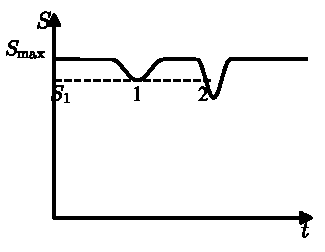
\includegraphics[width=4.5cm]{fig1.pdf}\\[0.3em]{\small 图 1}\end{minipage}\par\nopagebreak

但是，这样的说法当然和熵增长定律毫无共同之处，根据熵增长定律，在自然界中所有实际存在的闭合系统的熵从来不会减小（除了十分微小的涨落而外).同时，正是熵增长定律的这种普遍表述完全为自然界中发生的一切现象所证实.必须强调指出：这种表述与本节开头所给出的表述绝不等价，这一点似乎很明白.假如要从一种表述得到另一种表述，就不得不引入观测者的概念，他在某一时刻人为地“制造”一个闭合系统，使得关于系统以前的行为的问题根本不存在；物理定律对观测者性质的这种依赖性当然是完全不能接受的.

这样表述的熵增长定律是否能由经典力学导出，值得怀疑.况且，由于经典力学方程的时间反演不变性，只能寻求推导熵的单调变化.为了要得到熵单调增长的定律，我们就不得不定义时间方向，将之取为熵在增长的方向.这样又发生问题，即要证明这样的热力学定义与量子力学定义等同（见下文).

在量子力学中情况有本质性的改变.大家知道，量子力学的基本方程——薛定谔方程——本身是时间反演对称的（只要也将波函数 $\psi$ 换为 $\psi^{*}$).这意味着：如果在某一时刻 $t=t_1$，波函数给定为 $\psi=\psi(t_1)$，并且根据薛定谔方程，在另一时刻 $t=t_2$ 它应当变成等于 $\psi(t_2)$，那么从 $\psi(t_1)$ 到 $\psi(t_2)$ 的变化是可逆的；换句话说，如果在初始时刻 $t=t_1$，$\psi=\psi^{*}(t_2)$，那么在 $t=t_2$ 时将有 $\psi=\psi^{*}(t_1)$.不过，尽管有这种对称性，其实量子力学实际上含有两个时间方向的非等价性，这种非等价性的出现起因于量子力学中的基本过程即在量子客体与足够精确地服从经典力学的系统之间的相互作用过程.也就是说，如果同给定的一个量子客体依次发生两个相互作用过程（我们称它们为 A 和 B)，那么只有在过程 A 发生于过程 B 以前的情形下，才能够断言：过程 B 的某一结果的概率是取决于过程 A 的结果的（也可参阅本教程第三卷§7).

因此，在量子力学中，原则上，时间的两个方向具有物理上的非等价性，而熵增长定律很可能就是这种不等价性的宏观表现形式.在这种情况下必定存在一个含有量子常数 $\hbar$ 的不等式，以保证这个定律的正确性并在现实世界中得到实现.但是，直到目前任何人都未能以多少令人信服的方式探索这种联系并证明其确实存在.

因此，有关熵单调增长的物理基础的问题仍未解决.有没有它的宇宙学本质的起源？它与宇宙学中初始条件的普遍问题有没有联系？在基本粒子某些弱相互作用过程中时间反演对称性的破坏有没有什么贡献？很可能，只有在进一步综合物理学理论的过程中，才会对这样的问题求得答案.

作为总结，我们重述一下熵增长定律的普遍表述：在所有存在于自然界的闭合系统中，熵从来不会减少——它总是增长或者在极端情况下保持常数.相应于这两种可能性，通常把所有发生在宏观物体中的过程分为不可逆的和可逆的两种.前者指的是与整个闭合系统的熵增长相伴的过程，按照相反次序重复的过程是不可能发生的，因为在这种情况下熵不得不减少.如果闭合系统的熵在过程中保持常数\footnote{应当着重指出：这时系统中各个部分的熵未必也保持常数.}，因而过程也可以按相反的方向进行，那么这一类过程就称为可逆过程.自然，严格的可逆过程是理想的极限情形；实际上，在自然界中所进行的过程仅仅在一定的精度下才是可逆的.
